\chapter{Spintronique moléculaire}

\section{Spintronique et Électronique moléculaire}
Petit blabla introductif.
\subsection{La spintronique}
La spintronique est une branche de l'électronique où, en plus de la charge, le degré de liberté du spin est utilisé. Elle est notamment à l'origine des avancés technologiques les plus récentes telle que la MRAM ou bien encore les têtes de lecture des disque durs. Une des applications les plus célèbre reste la vanne de spin. Ce dispositif permet de filtrer les électrons en fonction de l'orientation de leur spin (soit \textit{up}, soit \textit{down}), autorisant un couplage direct entre magnétisme et courant. La découverte du phénomène de magnétorésistance géante, à l'origine de ce filtrage, a d'ailleurs value à ces découvreurs, Albert Fert et Peter Grünberg, le prix Nobel de Physique en 2007.


Ces applications technologique restent cependant cantonnées au stockage de  l'information~\cite{Awschalom2007}. Des propositions de spin-transistor directement commandé par le spin de l'électron et non plus sa charge ont pourtant été faites~\cite{Datta1990} et certains dispositifs ont également été réalisé~\cite{Johnson1996,Huang2007}.

Cependant, l'électron n'est pas le seul objet possédant un spin et d'autre "acteurs" de la spintronique peuvent être envisagée. Les aimants moléculaire, notamment du fait de l'emmergence de l'électronique moléculaire, sont des candidats sérieux dans la fabrication de dispositifs toujours plus performants. Avant de voir comment ces derniers pourrait \^etre utilisés dans l'électronique de demain, nous allons définir ce qu'est réellement un aimant moléculaire et quelles sont ces caractéristiques.

\section{L'électronique moléculaire}
Si une partie des développement de l'électronique s'est consacré à l'utilisation du degré de spin de l'électron, ce n'est néanmoins pas le seul axe de recherche de la discipline. Devant la recherche toujours plus grande de la miniaturisation des dispositifs, les chercheurs et les industriel se sont vite rendu compte des limites des technique de fabrication traditionnelle que l'on nomme parfois Top-Down. Elles consistes à partir d'un matériaux massif et de graver en son sein les structures nanométrique nécessaire à la production de l'électronique actuelle.




\section{Les aimants moléculaires}
\subsection{Définition}

Un molécule, pour recevoir le qualificatif d'aimant, doit remplir deux critères. Tout d'abord, elle doit posséder un moment magnétique. Celui-ci résulte, en général, de l'interaction entre plusieurs centres magnétiques et donne lieux à un configuration où la résultante des moments magnétiques des différents centres est non nulle. 

Il faut en outre que ce moment magnétique ait une orientation préférentielle, le long de laquelle il va venir s'aligner. Les deux directions associées à cette orientation représente les deux configuration d'énergie minimale séparé par une barrière de potentiel. Afin qu'un aimant moléculaire conserve ses propriétés, il faut que l'énergie associé à l'agitation thermique soit plus faible que cette barrière. Dans le cas contraire, la température suffit à retourner aléatoirement le moment magnétique.

Certains aimants moléculaire, en plus de l'axe facile, possèdent également un plan difficile dans lequel l'énergie du moment magnétique est la plus grande. Cela donne naissance à une physique beaucoup plus riche de part l'apparition de phénomènes quantiques tels que le retournement de l'aimantation par effet tunnel~(QTM) ou bien encore la phase de Berry, que nous détaillerons dans la suite.

Malgré ces restrictions, la zoologie des aimants moléculaires est plutôt riche avec des moments magnétique allant de un à plusieurs dizaines $\mu_B$.


\subsection{Propriétés}
Les aimants moléculaires possèdent de nombreuses propriétés susceptibles de les rendre indispensable aux dispositifs électroniques de demain. Leur taille tout d'abord, en deçà des techniques lithographique, permettrait d'augmenter les densités de stockage, chaque molécule codant une information à travers l'orientation de son moment magnétique. Un telle application est notamment motivé par le faible taux de relaxation, de l'ordre de quelques années en dessous de $2\,K$, qui permettrait d'en faire des éléments de stockage de l'information fiable.

De plus, certains aimant moléculaires peuvent être sensible à un stimulus extérieur tels que la température, la lumières, la pression, un champ électrique ou magnétique ou bien encore un déplacement de charge. Ils peuvent ainsi osciller entre deux configurations magnétiques différentes : "haut spin" et "bas spin". Ces interrupteurs moléculaires pourraient également constituer le composant élémentaires des mémoires de demain.

Les aimants moléculaires peuvent également jouer un rôle non négligeable dans l'information quantique. Cette dernière vise à utiliser les propriétés des systèmes quantiques afin d'obtenir des algorithmes plus efficaces pour la factorisation des nombres premiers~(avec des applications dans la cryptographie notamment) ou bien encore la recherche dans les bases de données. Des phénomènes quantiques tels le QTM ou bien la phase de Berry pourrait être utilisé dans ce cadre.

Nous allons maintenant illustrer certaines de ces propriétés à travers l'exemple d'un aimant moléculaire bien connu le octanuclear fer(III) oxo-hydroxo cluster dont la formule est [Fe$_8$O$_2$(OH)$_{12}$(tacn)$_6$]$^{8+}$ ou Fe$_8$.

\subsection{L'exemple du Fe$_8$}

\begin{figure}
\centering 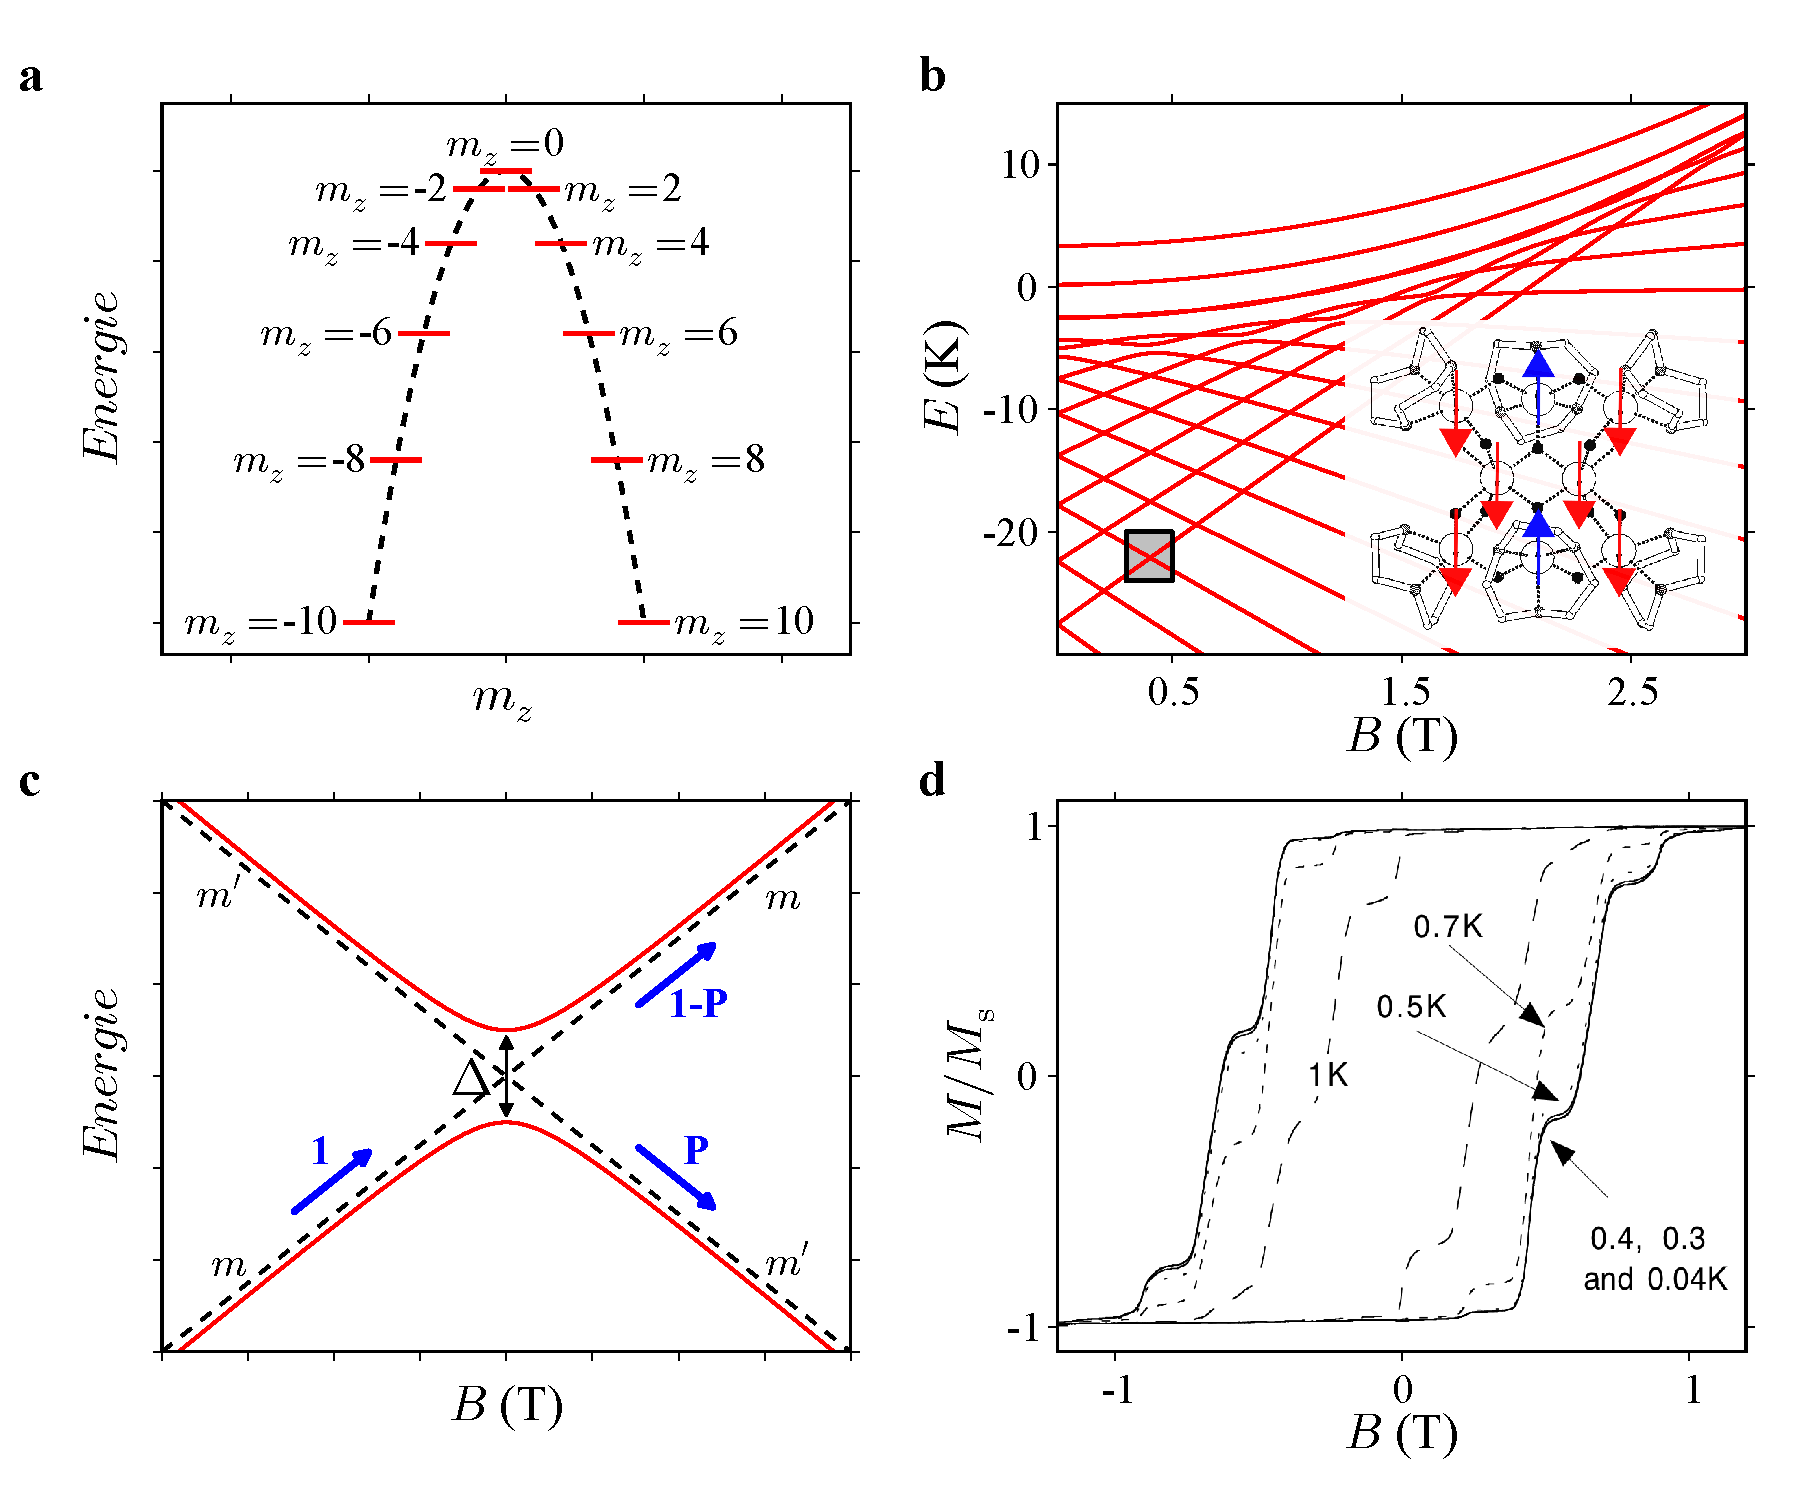
\includegraphics[scale=0.45]{Spintronique/FigureFe8/FigureFe8.pdf} 
\caption{\textbf{a} : énergie en fonction du nombre quantique $m_z$. Les deux orientations $m_z=\pm 10$ sont séparées par une barrière d'énergie de hauteur $|D|S^2$~\cite{Bogani2008}. \textbf{b} : diagramme Zeeman de la molécule Fe$_8$ représentant l'énergie des différents états du système en fonction du champ magnétique. Certains croisements, comme celui marqué d'un carré, sont en fait des anti-croisements traduisant un couplage entre les états. \textbf{c} : anti-croisement représentant un couplage entre les états $m$ et $m'$. \textbf{P} est la probabilité de transition entre les états $m$ et $m'$ lorsque l'on balaie l'anti-croisement en champ magnétique. \textbf{c} : mesure de l'aimantation d'un cristal de Fe$_8$ obtenue par technique micro-squid pour différentes températures. Les anti-croisements sont visibles à travers les marches qui traduisent un renversement de l'aimantation d'un grand nombre de molécules pour des valeurs particulières du champ magnétique~(extrait de \cite{MagGoesNano}).}
\label{Fe8Zeeman}
\end{figure}


Le Fe$_8$ se compose de huit atomes de fer de degré d'oxydation III, chacun de ces atomes constituant un centre magnétique de spin 5/2. De part les différentes interactions qui les lient, ils adoptent la configuration présenté dans la Fig.\ref{Fe8Zeeman}.\textbf{b} en encart avec un moment résultant total de $S=10$, le moment magnétique des deux atomes centraux se trouvant dans la direction opposée aux six atomes latéraux.

Les propriété magnétique de ce système peuvent \^etre décrite par l'hamiltonien suivant :
\begin{eqnarray}
H =  -DS_z^2 + \frac{E}{2} ( S_+^2  + S_-^2) + g\mu_b B S_z 
\end{eqnarray}
où $D$ est le paramètre d'anisotropie axiale, $E$ est le paramètre d'anysotropie transversale, $S_z$ et la projection sur $z$ du moment magnétique et $S_+$ et $S_-$ les opérateurs création anhilation.

A champ magnétique nul, les différents états magnétiques de la molécule se trouvent de part et d'autre d'un puit de potentiel, les deux états de plus basses énergie, $m_z=\pm10$ étant séparé par une énergie $D|S|^2$ où $S$ est le moment magnétique de la molécule (cf Fig.\ref{Fe8Zeeman}.\textbf{a}). Si l'énergie associé à l'agitation thermique est telle que $k_BT \ll D|S|^2$, l'aimantation de la molécule est parfaitement définie et aligné le long de l'axe $z$. Elle peut alors avoir deux orientation : \textit{up} lorsque $m_z=+10$ et \textit{down} lorsque $m_z=-10$.

Lorsque l'on applique un champ magnétique, l'énergie associée aux différents états du système va évoluer. On peut représenter cette évolution à l'aide d'un diagramme Zeeman dans lequel on représente l'énergie de chaque niveau en fonction du champ magnétique. La Fig.\ref{Fe8Zeeman}.\textbf{b} présente le digramme Zeeman associé au Fe$_8$ pour un champ magnétique allant jusqu'à $3\,T$. Un tel diagramme comporte de nombreux croisements pour lesquels deux états du système sont dégénérés.

Cependant, la présence d'un plan difficile introduit un couplage entre certains états du système. Quand ceux-ci sont en résonance~(i.e. ont la m\^eme énergie), le couplage est maximal, ce qui se traduit dans le diagramme Zeeman par ce que l'on appelle un anti-croisement. C'est notamment le cas de l'anti-croisement repéré par un rectangle dans la Fig.\ref{Fe8Zeeman}.\textbf{b}. La Fig.\ref{Fe8Zeeman}.\textbf{c} propose une vision schématique de ce dernier où $m$ et $m'$ sont les états du système loin de la résonance, $\Delta$ désigne la séparation en énergie entre les deux états et la ligne pointillé représente le diagramme Zeeman en l'absence de plan difficile.

Lorsque l'on balaie le champ magnétique autour d'un tel anti-croisement, il y a une certaine probabilité de passer de l'état $m$ à l'état $m'$ et vice-versas. Cette probabilité est régie par la formule de Landau-Zener~\cite{Zener1932} qui dépend à la fois de la séparation minimale entre les deux niveaux~$\Delta$, ainsi que de la vitesse de balayage du champ magnétique~$\frac{dB_z}{dt}$. Cette probabilité peut s'exprimer de la façon suivante :
\begin{eqnarray}
P = 1 - \exp \left( -\frac{\pi \Delta^2}{2 \hbar g \mu_B |m-m'|\frac{dB_z}{dt}} \right)
\end{eqnarray}
ou P est la probabilité de passer de l'état $m$ à l'état $m'$. On constate tout d'abord que si la vitesse est très faible, la probabilité de passer d'un état à l'autre tend vers 1. On retrouve ici le théorème adiabatique. A l'autre bout de l'échelle, si je balaie très rapidement le champ magnétique cette probabilité tend vers zéro. Tout se passe comme si le système n'avait pas eu le temps de "sentir" l'anti-croisement.


C'est lorsque le champ magnétique balaie un anti-croisement que le phénomène de QTM pourra être observé. En effet, le système pourra alors passé d'un coté de la barrière sans avoir à fournir l'énergie correspondante. Autrement dit, le renversement va se faire par effet tunnel à travers la barrière le potentiel, d'où le nom de renversement de l'aimantation par effet tunnel~(Qantum Tunneling of the Magnetization ou QTM en anglais).

Ce phénomène quantique peut être mise en évidence par une mesure de l'aimantation d'une assemblé de molécule. Une telle mesure consiste à relever l'aimantation d'un cristal moléculaire en fonction du champ magnétique. L'aimantation du cristal est d'abord amenée à saturation par l'application d'un fort champ magnétique. Celui-ci est ensuite balayé jusqu'à obtenir la saturation du cristal dans la direction opposée. Lorsque l'aimantation des molécules composant le cristal se retourne, elles modifient les lignes de champ environnante. De telle variation peuvent \^etre mesuré par une technique de micro-SQUID. La Fig.\ref{Fe8Zeeman}.\textbf{d} présente la mesure de l'aimantation d'un cristal de Fe$_8$ pour différentes températures et pour une vitesse de balayage de $14\,mT.s^{-1}$.

La courbe montre une série de marches qui sont d\^ues au retournement par QTM. Chacune d'elles correspond à un anti-croisement sur lequel l'aimantation à une probabilité élevée de transiter. Lorsque l'on diminue la température, le taux de retournement diminue car les transitions assistées thermiquement diminuent. Cette courbe devient indépendante de la température au dessous de 400\,mK et on observe les transitions correspondantes aux niveaux de plus basse énergie. 

\section{La spintronique moléculaire}
La spintronique moléculaire a pour but de combiner les techniques de la spintronique avec les nouveaux développement de l'électronique moléculaire et de la chimie, afin de produire de nouveaux dispositif susceptible de compléter ou éventuellement remplacé les technologies tout semi-conducteurs. Cette discipline a connue une évolution fulgurante ces dernières années, bénéficiant des dernière avancé en matière de lithographie, mais aussi de la mise en synergie du travail des physiciens et des chimistes. 

Dans ce paragraphe, je ne présenterai bien sûr qu'une partie des nombreux travaux effectués dans le domaine. Ceci ne constitue donc en aucun cas une liste exhaustive des expériences réalisées, ni m\^eme une liste des plus cruciales. Elle permettrons néanmoins, je l'espère, d'aider le lecteur à situer nos travaux par rapport aux recherchent en cours dans d'autres laboratoires. De plus, je me limiterai ici au dispositif ne comportant qu'un nombre limités de molécules, de l'ordre de l'unité, généralement utilisé dans les laboratoires de recherche fondamentale.
\subsection{État de l'art}

\subsubsection*{Du premier transistor moléculaire...}
La première expérience de mesure de courant à travers une molécule unique a été faite en 1995 à l'aide un microscope à effet tunnel ou STM. Il s'agissait de mesurer la resistance à travers une molécule de C$_{60}$ déposé sur une surface d'or. Il ne s'agissait pas encore dans ce cas d'une structure de type transistor, puis seul deux terminaux sont présent à savoir, le surface conductrice et la point du STM.

Cette expérience, et celles qui ont suivi, ont encouragé le développement de nouvelles technique permettant de piéger une molécule unique dans un dispositif de mesure. C'est ainsi qu'est apparu la technique dite de "break junction". Elle consiste à suspendre un fin pont métallique puis à plier le support jusqu'à obtenir une cassure. La taille de celle-ci peut être ensuite modulée en faisant varier la courbure imposée à l'échantillon. A l'aide de ce dispositif, Reed et collègues ont pu mesurer, en 1995, des molécules de benzene-1,4-dithiol et montrer l'influence du couplage électrique entre les deux électrodes et la molécule sur la conductance mesurée. Cette technique présente cependant l'inconvénient de ne pas avoir de grille m\^eme si celui a été partiellement corrigé par l'ajout de grille sans cependant obtenir un couplage satisfaisant.

Pour disposer enfin d'une grille permettant de moduler le potentiel, et donc l'état de charge, de la molécule piégée, il a fallu attendre encore 5 ans et la réalisation du premier transistor à molécule unique. Celui-ci consistait en un atome de C$_{60}$ piégé entre deux électrode d'or et un grille. Ce dispositif a été obtenue en faisant circuler une forte densité de courant dans un fil fin d'or, venant provoquer la migration des atomes au niveau du point faible et provocant une cassure de l'ordre du nanomètre. Le phénomène d'électromigration est un phénomène bien connu des micro-électroniciens puisqu'il est à l'origine de certaines défaillance dans les puces et autres dispositifs électroniques. Il a d'ailleurs donné son nom à la technique : l'électromigration. Nous présenterons cette dernière plus en détail dans le chapitre consacré à la fabrication de notre échantillon, puisque c'est également cette technique que nous avons utiliser dans le cadre de nos travaux. L'expérience menée sur ce premier transistor moléculaire avait pu mettre en évidence le couplage entre les vibrations moléculaires et la résistance du dispositif. De plus la grille se révélait suffisamment efficace pour modifier l'état de charge de la molécule de C$_{60}$ permettant ainsi d'obtenir les premiers diamants de Coulomb associé à une molécule unique.

Cependant, dans ces dispositifs, aucune propriété propre aux molécules n'est utilisé et le seul spin en jeux dans les phénomènes reste celui de l'électron. Hors, l'avantage principal des molécules, outre leur taille, provient des différentes propriété, notamment magnétique, que la chimie moderne peut leur  conférer.

\subsubsection*{\`A la véritable spintronique moléculaire}

L'année 2006 a vu paraître les deux première expérience visant à insérer des aimants moléculaires au sein d'un gap afin d'obtenir les premiers dispositif de spintronique moléculaire. La première a été publié par le groupe de H.S.J van der Zant et la seconde par le groupe de D.C. Ralph, et portaient toute deux sur l'étude d'un aimant moléculaire bien connu : le Mn$_{12}$. Un des aspect intéressant de ces expériences, outre le magnétisme de la molécule, est la fonctionnalisation de cette dernière à l'aide de groupe thiol, afin de favoriser le couplage avec les électrodes d'or de la source et du drain. Cela illustre la souplesse de la chimie et la possibilité qu'elle offre de fabriquer des molécules faites sur mesure afin de faciliter certaines configurations ou certain comportement~(ici une forte affinité avec l'or).  

Cependant, les mesures en transport, bien que montrant une dépendence en champ magnétique complexe et des signe de conductance différentielle négative, n'ont pas permis de confirmer, de façon certaine, s'il s'agissait bien d'un molécule de Mn$_{12}$, ni même de savoir si les propriété magnétique de cette dernière avait été conservées durant la fabrication. Le groupe de D.C. Ralph conclue d'ailleurs ses travaux par la phrase suivante : ``We find significant variations between devices, indicating that the sample fabrication process and the device environment may affect our molecules".

La première expérience réellement convaincante de transistors moléculaires mettant en jeux une molécule magnétique a été réalisée en 2008 dans le groupe de D.C. Ralph. Toujours avec la technique d'électromigration, ils avaient produit un transistor dont les électrodes était en platine, la grille locale était en oxyde d'aluminium et le rôle du canal était donc joué par une molécule de N@C$_{60}$. Il avait alors pu mettre en évidence le magnétisme lié à l'atome d'azote de spin S=3/2 à travers de mesure en transport et remonté au couplage entre ce dernier et les électrons de la cage de C$_{60}$. 

Il s'agit, à mes yeux, du premier dispositif que l'on peut qualifier de spintronique moléculaire à l'échelle de la molécule unique. En effet, les propriétés magnétique de la molécule isolé se retrouve de façon non-équivoque dans mes mesures en transport. Ce n'est d'ailleurs pas surprenant car fort de leur expérience avec le Mn$_{12}$ les auteurs avait choisi le N@C$_{60}$ pour la robustesse de sa structure et de ces propriétés magnétique comme ils le précisent dans leur papier. Cependant, bien que possédant un moment magnétique, cette dernière n'appartient pas à la catégorie des aimants moléculaire. En effet, elle ne possède pas d'axe facile et l'orientation de son moment magnétique n'est déterminé que par le champ magnétique.

Loin d'\^etre des échecs, ces différents travaux ont fournis un apport important au reste de la communauté notamment concernant les critères essentiels que doivent remplir les aimants moléculaire susceptible d'être étudié par les techniques expérimentales actuelles. Je détaillerai ces différents critères lorsque j'introduirai le Terbium double-Decker, en les mettant en relation avec les différents article.
 
\subsection{La spintronique dans notre groupe}
Le groupe au sein duquel j'ai effectué ma thèse a une culture ancré dans le nano-magnétisme et le magnétisme moléculaire. Une bonne partie des efforts de la fin des année 1990 et du début des années 2000 a été consacré à l'analyse et la caractérisation de système magnétique allant de la nanoparticule au cristal moléculaire en passant par l'aimant moléculaire isolé et le spin nucléaire unique. A chaque échelle de mesure correspond un appareil de mesure, et assez logiquement, plus le système à mesuré est petit, plus le détecteur l'est également. Cette tendance est bien représenté dans la figure??. Pour des particule macroscopique, l'usage d'un squid est suffisant. Lorsque l'on veut caractérisé des particules de l'ordre de quelques dizaines de nanomètre ou bien encore un cristal moléculaire, l'usage d'un détecteur aussi sensible qu'un micro-squid est indispensable.

Lorsque l'objet a détecter devient très petit, comme une molécule par exemple, il n'est plus vraiment possible de faire la distinction entre le détecteur et l'objet à mesurer. Il faut alors songer à fabriquer un dispositif électronique dont le fonctionnement même est influencé par le magnétisme de l'un de ces composant. Autrement dit, il faut faire appel à la spintronique et plus précisement, lorsque l'on s'intéresse au molécule, à la spintronique moléculaire.